\begin{figure}[H]
\centering
\shorthandoff{<>}
\begin{minipage}[t]{0.48\linewidth}
\centering
\textbf{(a) Distribución de alturas}

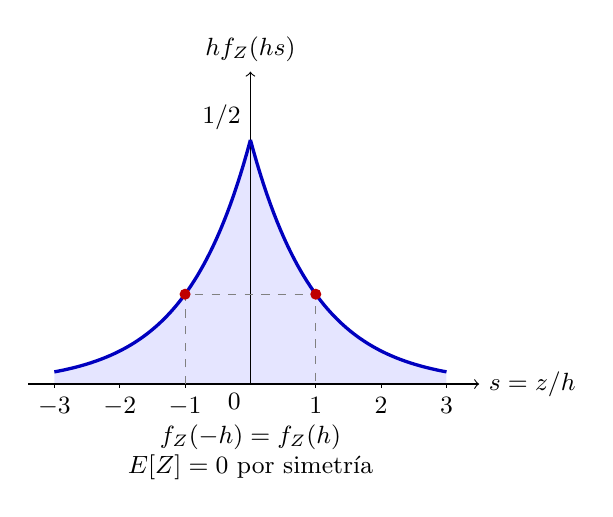
\begin{tikzpicture}[x=0.83cm,y=6.2cm,font=\small]
  \fill[blue!10] (-3,0) -- plot[domain=-3:0,samples=60,variable=\heightvalue]
    ({\heightvalue},{0.5*exp(\heightvalue)})
    -- plot[domain=0:3,samples=60,variable=\heightvalue]
    ({\heightvalue},{0.5*exp(-\heightvalue)}) -- (3,0) -- cycle;
  \draw[->] (-3.4,0) -- (3.5,0) node[right] {$s=z/h$};
  \draw[->] (0,0) -- (0,0.64) node[above] {$h f_Z(hs)$};
  \draw[blue!75!black,very thick] plot[domain=-3:0,samples=60,variable=\heightvalue]
    ({\heightvalue},{0.5*exp(\heightvalue)});
  \draw[blue!75!black,very thick] plot[domain=0:3,samples=60,variable=\heightvalue]
    ({\heightvalue},{0.5*exp(-\heightvalue)});
  \draw[dashed,gray] (-1,0) -- (-1,0.18394) -- (1,0.18394) -- (1,0);
  \fill[red!75!black] (-1,0.18394) circle (2pt);
  \fill[red!75!black] (1,0.18394) circle (2pt);
  \node[above left] at (0,0.5) {$1/2$};
  \foreach \tick in {-3,-2,-1,1,2,3}{
    \draw (\tick,0) -- (\tick,-0.008) node[below] {$\tick$};
  }
  \node[below left] at (0,0) {$0$};
  \node[align=center] at (0,-0.14) {$f_Z(-h)=f_Z(h)$\\$E[Z]=0$ por simetría};
\end{tikzpicture}
\end{minipage}\hfill
\begin{minipage}[t]{0.48\linewidth}
\centering
\textbf{(b) Transformación cuadrática}

\begin{tikzpicture}[x=1.05cm,y=0.95cm,font=\small]
  \draw[->] (-2.35,0) -- (2.5,0) node[right] {$s=z/h$};
  \draw[->] (0,0) -- (0,4.2) node[above] {$x=\dfrac{r-R_0}{\alpha h^2}$};
  \draw[blue!75!black,very thick] plot[domain=-1.9:1.9,samples=100,variable=\heightvalue]
    ({\heightvalue},{\heightvalue*\heightvalue});
  \draw[red!75!black,dashed] (-2.1,1) -- (2.1,1) node[right] {$x=1$};
  \draw[dashed,gray] (-1,0) -- (-1,1);
  \draw[dashed,gray] (1,0) -- (1,1);
  \fill[red!75!black] (-1,1) circle (2pt);
  \fill[red!75!black] (1,1) circle (2pt);
  \foreach \tick in {-2,-1,1,2}{
    \draw (\tick,0) -- (\tick,-0.05) node[below] {$\tick$};
  }
  \node[below left] at (0,0) {$0$};
  \node at (0.9,3.4) {$x=s^2$};
  \node[align=center] at (0,-0.9) {$z=-h$ y $z=h$ producen\\el mismo $r=R_0+\alpha h^2$};
\end{tikzpicture}
\end{minipage}
\shorthandon{<>}
\caption{La distribución de alturas es simétrica respecto al plano galáctico. Dos alturas opuestas producen el mismo radio efectivo; los puntos rojos ilustran el caso $z=\pm h$. Por ello, ambas alturas deben contribuir al cálculo de $g(r)$. Los ejes están expresados en variables adimensionales.}
\label{fig:altura-transformacion}
\end{figure}